\documentclass[11pt,a4paper]{article}

\usepackage[utf8]{inputenc}
\usepackage[T1]{fontenc}
\usepackage{graphicx}
\usepackage{booktabs}
\usepackage{tabularx}
\usepackage{amsmath,amssymb}
\usepackage{geometry}
\usepackage{caption}
\usepackage{subcaption}
\usepackage{listings}
\usepackage{enumitem}
\usepackage{fancyhdr}
\usepackage{hyperref}
\usepackage{xcolor}
\usepackage{microtype}
\usepackage{float}
\setlength{\emergencystretch}{3em}

\geometry{margin=2.5cm}

\hypersetup{
  colorlinks=true,
  linkcolor=blue!60!black,
  citecolor=blue!60!black,
  urlcolor=blue!60!black,
}

\captionsetup{font=small,labelfont=bf}
\setlist{nosep,leftmargin=1.4em}

\lstset{
  basicstyle=\ttfamily\small,
  breaklines=true,
  frame=single,
  numbers=left,
  numbersep=5pt,
  showstringspaces=false,
}

\pagestyle{fancy}
\fancyhf{}
\fancyhead[L]{\small Data Mining: Fundamental}
\fancyhead[R]{\small Seller-Level Vehicle Listings}
\fancyfoot[C]{\thepage}
\renewcommand{\headrulewidth}{0.4pt}

%=====================================================================
%  Project metadata -- EDIT THESE
%=====================================================================
\newcommand{\coursename}{DATA MINING: FUNDAMENTAL}
\newcommand{\projecttitle}{Project report: Seller-Level Vehicle Listings Dataset}
\newcommand{\academicyear}{Academic Year 2026/2027}
\newcommand{\teacherA}{Dino Pedreschi}
\newcommand{\teacherB}{Riccardo Guidotti}
\newcommand{\teacherC}{Alessio Cascione}
\newcommand{\memberA}{Muhammad Iqbal Zain}
\newcommand{\memberB}{Truong Giang Do}
\newcommand{\memberC}{Vladislav Zhelezov}

\begin{document}

%---------------------------------------------------------------------
%  Title page
%---------------------------------------------------------------------
\begin{titlepage}
  \centering
  \vspace*{1cm}
  
\includegraphics[width=0.28\linewidth]{figures/unipi_logo.png}\\[1.2cm]
  {\Large UNIVERSITY OF PISA}\\[0.3cm]
  {\large DEPARTMENT OF COMPUTER SCIENCE}\\[0.8cm]
  {\large Master programme in Data Science and Business Informatics}\\[2.5cm]
  {\LARGE\bfseries \coursename}\\[0.6cm]
  {\Large \projecttitle}\\[3.5cm]
  \begin{minipage}[t]{0.45\linewidth}
    \raggedright
    Teachers:\\
    \teacherA\\
    \teacherB\\
    \teacherC
  \end{minipage}\hfill
  \begin{minipage}[t]{0.45\linewidth}
    \raggedleft
    Group:\\
    \memberA\\
    \memberB\\
    \memberC
  \end{minipage}\\[3cm]
  \rule{\linewidth}{0.4pt}\\[1cm]
  {\large \academicyear}
\end{titlepage}

%---------------------------------------------------------------------
\pagenumbering{roman}
\tableofcontents
\newpage

%=====================================================================
\pagenumbering{arabic}
\section{Data Understanding and Preparation}
\label{sec:understanding}
The dataset analyzed in this section comprises 13,843 records across 33 features. Each record represents an individual seller profile identified by \texttt{sp\_id}, aggregating inventory and listing-level attributes associated with that seller.

In this section, we explore the data by examining feature semantics and distributions, identifying potential outliers, and outlining our strategy for handling missing values.

\subsection{Data semantics}
\label{sec:semantics}
\emph{The Seller-Level Vehicle Listings Dataset} contains one record per seller (\texttt{sp\_id}), summarising the vehicle listings observed for that seller. The meaning, source datatype and measurement scale of each variable are reported in Table~\ref{tab:semantics}. The prediction target is \texttt{seller\_rating\_class} (low/medium/high).

\begin{table}[htbp]
  \centering
  \caption{Semantic description of the dataset variables.}
  \label{tab:semantics}
  \footnotesize
  \setlength{\tabcolsep}{4.5pt}
  \renewcommand{\arraystretch}{1.1}
  \begin{tabularx}{\textwidth}{l X l l}
    \toprule
    Feature Name & Description & Datatype & Msrmt Scale \\
    \midrule
    \emph{sp\_id} & Unique identifier of the seller/dealer & float64 & Identifier \\
    \emph{n\_listings} & Total number of vehicle listings & int64 & Numerical \\
    \emph{price\_median} & Median advertised price of vehicles & float64 & Numerical \\
    \emph{savings\_amount\_median} & Median advertised savings amount & float64 & Numerical \\
    \emph{daysonmarket\_median} & Median days vehicles remained on market & float64 & Numerical \\
    \emph{mileage\_median} & Median vehicle mileage & float64 & Numerical \\
    \emph{year\_median} & Median vehicle model year & float64 & Numerical \\
    \emph{vehicle\_age\_median} & Median vehicle age at listing time & float64 & Numerical \\
    \emph{owner\_count\_median} & Median number of previous vehicle owners & float64 & Numerical \\
    \emph{horsepower\_median} & Median vehicle horsepower & float64 & Numerical \\
    \emph{engine\_displacement\_median} & Median vehicle engine displacement & float64 & Numerical \\
    \emph{city\_fuel\_economy\_median} & Median city fuel economy & float64 & Numerical \\
    \emph{highway\_fuel\_economy\_median} & Median highway fuel economy & float64 & Numerical \\
    \emph{back\_legroom\_median} & Median rear-seat legroom & float64 & Numerical \\
    \emph{front\_legroom\_median} & Median front-seat legroom & float64 & Numerical \\
    \emph{fuel\_tank\_volume\_median} & Median fuel tank capacity & float64 & Numerical \\
    \emph{height\_median} & Median vehicle height & float64 & Numerical \\
    \emph{length\_median} & Median vehicle length & float64 & Numerical \\
    \emph{width\_median} & Median vehicle width & float64 & Numerical \\
    \emph{pct\_isCab} & Proportion of vehicles previously used as cabs & float64 & Numerical \\
    \emph{pct\_is\_new} & Proportion of vehicles classified as new & float64 & Numerical \\
    \emph{pct\_salvage} & Proportion of vehicles with salvage status & float64 & Numerical \\
    \emph{pct\_theft\_title} & Proportion of vehicles with theft titles & float64 & Numerical \\
    \emph{n\_listing\_days} & Distinct calendar days with observed listings & int64 & Numerical \\
    \emph{listing\_span\_days} & Span in days between earliest and latest listing & int64 & Numerical \\
    \emph{dominant\_body\_type} & Most frequent vehicle body type & str & Categorical \\
    \emph{dominant\_fuel\_type} & Most frequent fuel type & str & Categorical \\
    \emph{dominant\_transmission} & Most frequent transmission type & str & Categorical \\
    \emph{dominant\_wheel\_system} & Most frequent drivetrain configuration & str & Categorical \\
    \emph{dominant\_listing\_color} & Most frequent exterior color & str & Categorical \\
    \emph{franchise\_status} & Franchise status (franchise, independent, etc.) & str & Categorical \\
    \emph{new\_used\_profile} & Inventory composition (new\_only, used\_only, etc.) & str & Categorical \\
    \emph{seller\_rating\_class} & Discretized target rating (low, medium, high) & str & Ordinal \\
    \bottomrule
  \end{tabularx}
\end{table}

\subsection{Distribution of variables and statistics}
\label{sec:distribution}
In this section, we summarise the data distributions to better understand each variable.

\subsubsection{Summary of statistics}
\label{sec:summary-stats}
This subsection summarises the statistical properties of each attribute in the dataset. In addition to the mean, standard deviation and quartiles obtained from \texttt{df.describe()}, we report the number of missing values, skewness, kurtosis and the interquartile range (IQR) for the 24 numerical columns. Table~\ref{tab:stats} gives a high-level view of the seller-level vehicle listings data.

The table shows that the features differ considerably in scale: the \texttt{pct\_*} proportions range from 0 to 1, whereas \texttt{mileage\_median} spans from 0 to 238k. This disparity indicates that the data should be standardised to a common scale before being used by models that are sensitive to feature magnitude.

The table also reveals that some features are strongly skewed while others are not, and that several columns contain missing values. Both observations motivate the cleaning and preparation steps discussed in the following subsections.

\begin{table}[htbp]
  \centering
  \caption{Summary statistics for the 24 numerical variables (identifier excluded).}
  \label{tab:stats}
  \footnotesize
  \setlength{\tabcolsep}{3pt}
  \renewcommand{\arraystretch}{1.05}
  \resizebox{\textwidth}{!}{%
  \begin{tabular}{lrrrrrrrrrrrr}
    \toprule
    Variable & Count & Mean & Std & Min & 25\% & 50\% & 75\% & Max & Missing & Skew & Kurtosis & IQR \\
    \midrule
n\_listings & 13843.0 & 118.10 & 137.06 & 5.00 & 25.00 & 70.00 & 168.00 & 4959.00 & 0 & 5.25 & 120.32 & 143.00 \\
    price\_median & 13843.0 & 23106.14 & 14365.07 & 1699.00 & 12495.00 & 22385.00 & 29888.00 & 236438.00 & 0 & 3.45 & 34.14 & 17393.00 \\
    savings\_amount\_median & 13843.0 & 446.21 & 519.46 & 0.00 & 0.00 & 358.00 & 734.00 & 9333.00 & 0 & 2.40 & 18.30 & 734.00 \\
    daysonmarket\_median & 13843.0 & 49.15 & 56.06 & 0.00 & 26.00 & 36.00 & 51.00 & 1987.00 & 0 & 8.75 & 168.60 & 25.00 \\
    mileage\_median & 13842.0 & 51463.27 & 51845.46 & 0.00 & 25.00 & 33596.50 & 96915.75 & 238541.00 & 1 & 0.68 & -0.77 & 96890.75 \\
    year\_median & 13843.0 & 2015.95 & 4.72 & 1960.00 & 2013.00 & 2017.00 & 2020.00 & 2021.00 & 0 & -2.25 & 14.09 & 7.00 \\
    vehicle\_age\_median & 13842.0 & 4.08 & 4.63 & 0.00 & 0.00 & 3.00 & 7.00 & 60.00 & 1 & 2.32 & 14.98 & 7.00 \\
    owner\_count\_median & 13804.0 & 1.43 & 0.62 & 1.00 & 1.00 & 1.00 & 2.00 & 6.00 & 39 & 1.30 & 1.35 & 1.00 \\
    horsepower\_median & 13837.0 & 240.90 & 56.99 & 78.00 & 188.00 & 243.00 & 283.00 & 630.00 & 6 & 0.85 & 2.05 & 95.00 \\
    engine\_displacement\_median & 10450.0 & 2925.08 & 808.08 & 1200.00 & 2400.00 & 2500.00 & 3500.00 & 6800.00 & 3393 & 1.29 & 2.77 & 1100.00 \\
    city\_fuel\_economy\_median & 13827.0 & 20.65 & 3.96 & 10.00 & 18.00 & 20.00 & 22.00 & 126.00 & 16 & 8.10 & 185.87 & 4.00 \\
    highway\_fuel\_economy\_median & 13827.0 & 27.88 & 3.98 & 15.00 & 25.00 & 27.50 & 30.00 & 105.00 & 16 & 3.88 & 66.79 & 5.00 \\
    back\_legroom\_median & 13824.0 & 37.71 & 1.57 & 0.00 & 36.80 & 37.80 & 38.60 & 47.50 & 19 & -3.53 & 77.81 & 1.80 \\
    front\_legroom\_median & 13836.0 & 41.89 & 0.77 & 36.60 & 41.30 & 41.80 & 42.20 & 67.00 & 7 & 3.49 & 88.62 & 0.90 \\
    fuel\_tank\_volume\_median & 13836.0 & 18.35 & 2.93 & 7.15 & 16.40 & 18.25 & 19.20 & 52.00 & 7 & 1.83 & 7.33 & 2.80 \\
    height\_median & 13837.0 & 65.15 & 4.95 & 46.85 & 61.60 & 66.00 & 68.00 & 107.50 & 6 & 0.18 & 0.91 & 6.40 \\
    length\_median & 13837.0 & 191.10 & 10.25 & 151.00 & 184.60 & 189.80 & 192.70 & 282.30 & 6 & 2.18 & 7.59 & 8.10 \\
    width\_median & 13837.0 & 77.02 & 4.97 & 65.70 & 72.90 & 75.55 & 80.00 & 105.90 & 6 & 1.06 & 1.56 & 7.10 \\
    pct\_isCab & 13816.0 & 0.16 & 0.16 & 0.00 & 0.05 & 0.12 & 0.21 & 1.00 & 27 & 2.04 & 5.91 & 0.17 \\
    pct\_is\_new & 13843.0 & 0.27 & 0.32 & 0.00 & 0.00 & 0.00 & 0.59 & 1.00 & 0 & 0.55 & -1.38 & 0.59 \\
    pct\_salvage & 13816.0 & 0.01 & 0.06 & 0.00 & 0.00 & 0.00 & 0.00 & 1.00 & 27 & 10.34 & 119.82 & 0.00 \\
    pct\_theft\_title & 13816.0 & 0.00 & 0.02 & 0.00 & 0.00 & 0.00 & 0.00 & 0.76 & 27 & 14.11 & 427.34 & 0.00 \\
    n\_listing\_days & 13843.0 & 46.32 & 33.72 & 1.00 & 18.00 & 39.00 & 68.00 & 272.00 & 0 & 0.98 & 0.95 & 50.00 \\
    listing\_span\_days & 13843.0 & 405.59 & 282.37 & 0.00 & 223.00 & 362.00 & 508.00 & 3553.00 & 0 & 2.15 & 9.00 & 285.00 \\
    \bottomrule
  \end{tabular}}
\end{table}

\subsubsection{Distribution via histograms}
\label{sec:histograms}
A histogram (Figure~\ref{fig:hist}) is used to visualise the distribution of the data. This method also helps to identify patterns, anomalies and skewness, and supports the statistics reported in Table~\ref{tab:stats}.

Since 24 numerical features are too many to show at this stage, we select a semantically representative subset of columns: \texttt{n\_listings}, \texttt{price\_median}, \texttt{daysonmarket\_median}, \texttt{mileage\_median}, \texttt{year\_median}, \texttt{owner\_count\_median}, \texttt{horsepower\_median}, \texttt{city\_fuel\_economy\_median}, \texttt{front\_legroom\_median}, \texttt{fuel\_tank\_volume\_median}, \texttt{height\_median} and \texttt{pct\_is\_new}.

\begin{figure}[htbp]
  \centering
  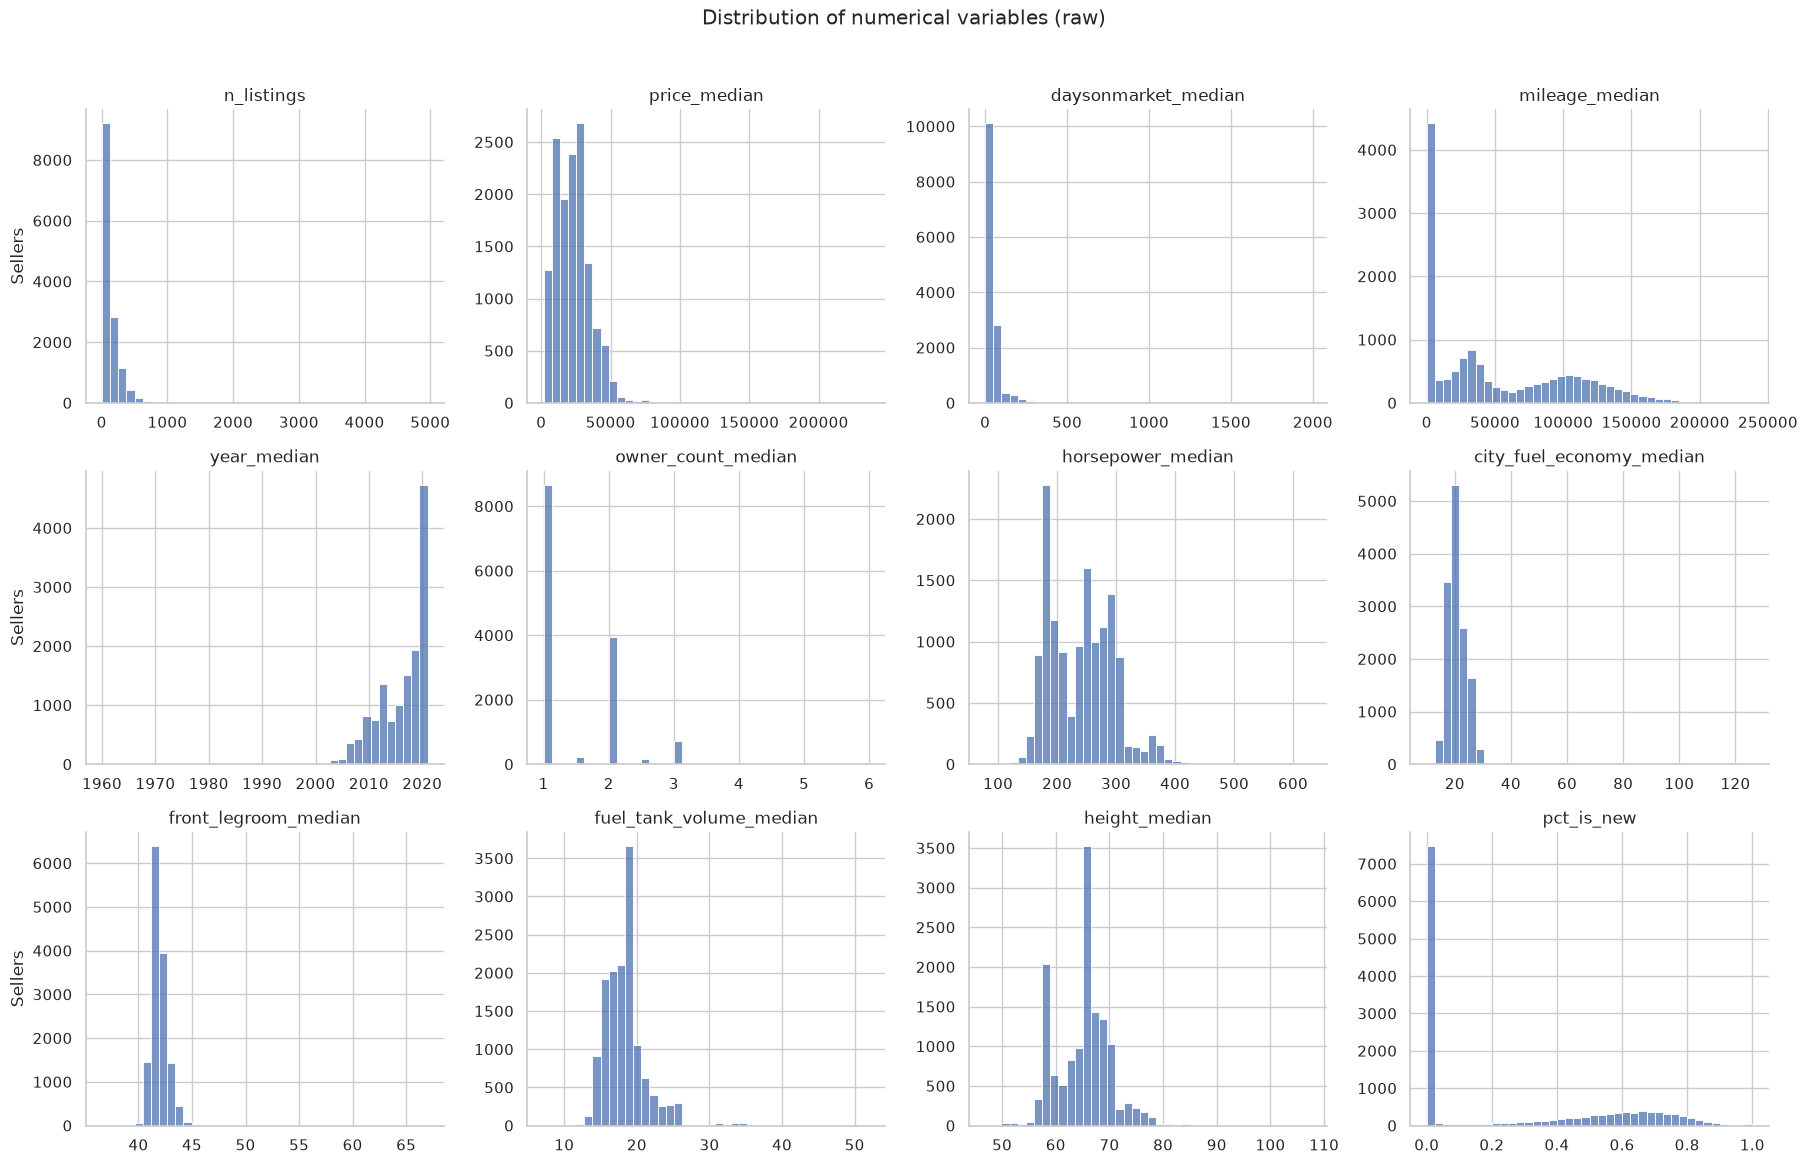
\includegraphics[width=\linewidth]{figures/fig_1_1_histograms.png}
  \caption{Histograms of the selected numerical variables.}
  \label{fig:hist}
\end{figure}

From the figure, most of the selected features are highly skewed, which is confirmed by the skewness values above 1 in Table~\ref{tab:stats}. Most sellers have fewer than 500 listings and stay on the market for fewer than 200 days. \texttt{pct\_is\_new} and \texttt{mileage\_median} show that many of the cars being sold are new and have never been driven, while \texttt{owner\_count\_median} indicates that most cars have had one or two previous owners.

The large empty space on the right side of several panels indicates extremely high (or low) outliers, which is also supported by the high kurtosis in Table~\ref{tab:stats}.

\subsubsection{Distribution of categorical features}
\label{sec:categorical}
To better understand the distribution of the categorical data, we use pie charts for low-cardinality features and bar charts for higher-cardinality features, where magnitudes are easier to compare. The pie charts are shown in Figure~\ref{fig:pie}, while the bar charts are shown in Figure~\ref{fig:bar}.

\begin{figure}[htbp]
  \centering
  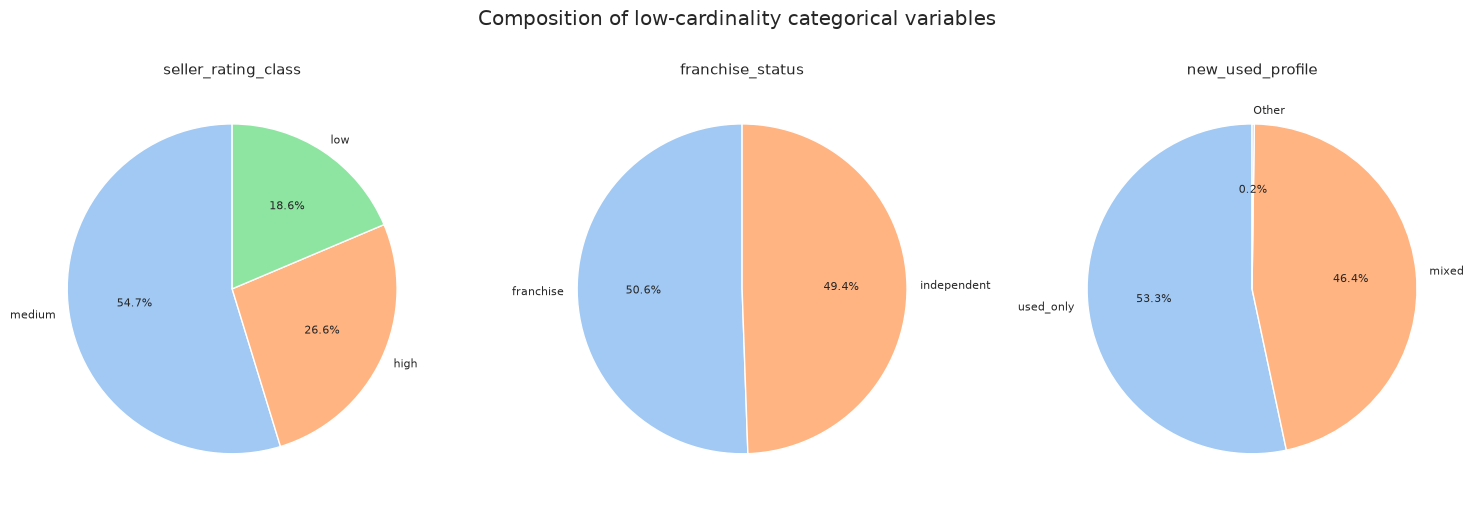
\includegraphics[width=\linewidth]{figures/fig_1_2_pie.png}
  \caption{Composition of the low-cardinality categorical variables.}
  \label{fig:pie}
\end{figure}

From the pie charts, \texttt{seller\_rating\_class} is dominated by the \textit{medium} class, followed by \textit{high}. In contrast, \texttt{franchise\_status} and \texttt{new\_used\_profile} are relatively well balanced across their values.

\begin{figure}[htbp]
  \centering
  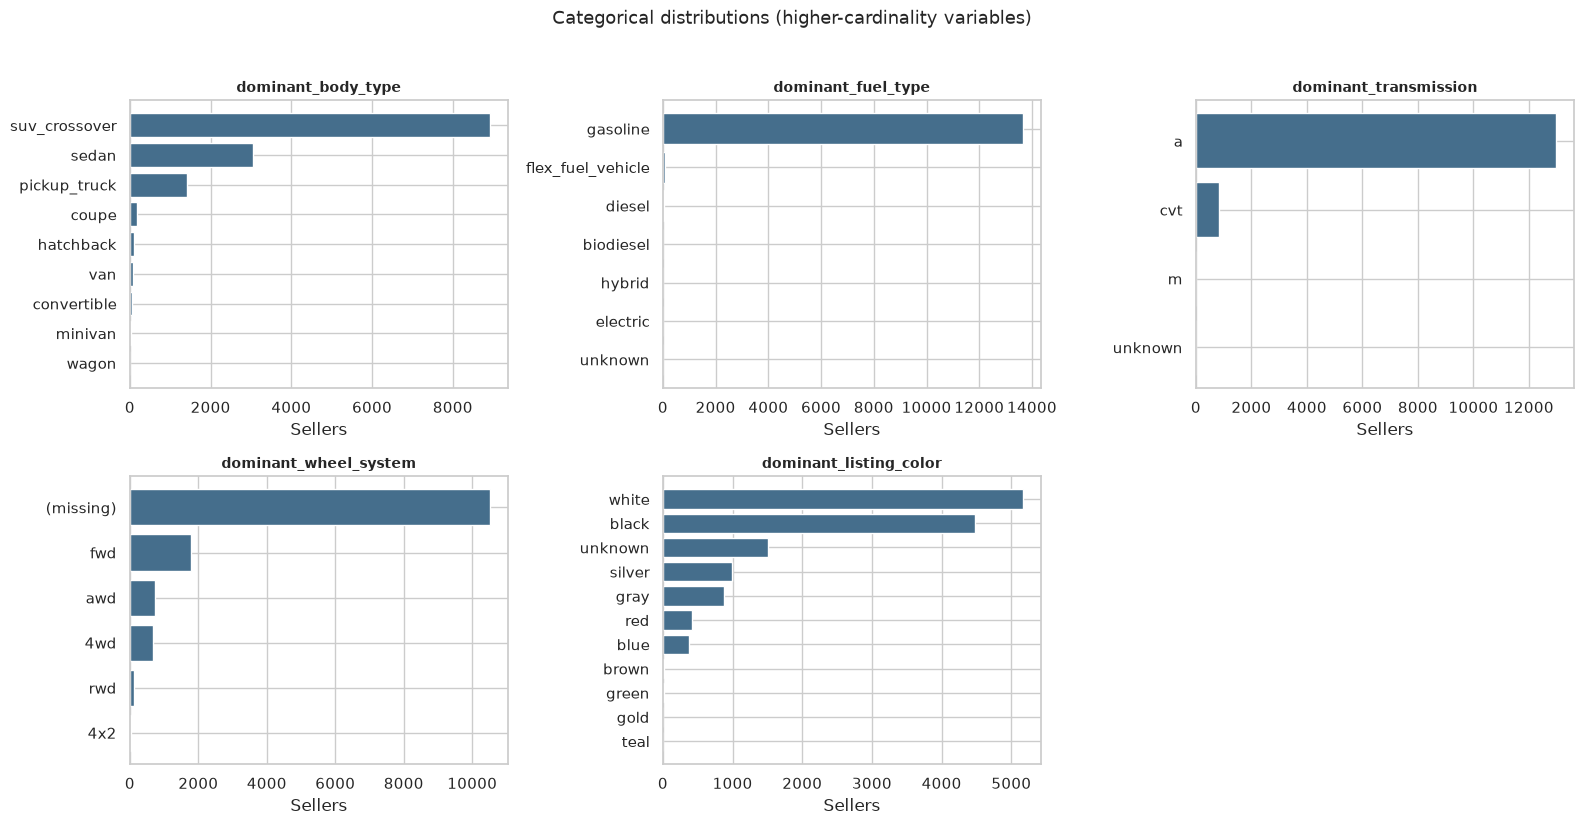
\includegraphics[width=\linewidth]{figures/fig_1_3_bar.png}
  \caption{Distributions of the higher-cardinality categorical variables.}
  \label{fig:bar}
\end{figure}

The bar charts show that the value \texttt{a} (automatic) dominates \texttt{dominant\_transmission}, while \texttt{dominant\_fuel\_type} is clearly dominated by \textit{gasoline}. For \texttt{dominant\_wheel\_system}, we include a \texttt{(missing)} value to highlight the large proportion of missing data. In \texttt{dominant\_listing\_color}, black and white are the most common colours, followed by \textit{unknown}; colours such as brown, green, gold and teal are present but represent only small fractions of the cars. Finally, SUVs account for a very large proportion of \texttt{dominant\_body\_type}, followed by sedans and pickup trucks; the remaining body types are present but not significant.

\subsection{Assessment of data quality}
\label{sec:quality}
Before statistical imputation and feature transformation, we ran a syntactic and semantic audit across the dataset. First, no duplicated rows were found, and the sellers' identifiers (\texttt{sp\_id}) are unique. Second, no negative values appear in any numerical attribute. Third, all percentage attributes (\texttt{pct\_isCab}, \texttt{pct\_is\_new}, \texttt{pct\_salvage}, \texttt{pct\_theft\_title}) are correctly bounded within the closed interval $[0,1]$, and advertised discounts never exceed the original prices (\texttt{savings\_amount\_median} $<$ \texttt{price\_median}). Moreover, temporal consistency holds across all records (\texttt{n\_listing\_days} $\leq$ \texttt{n\_listings} and \texttt{n\_listing\_days} $\leq$ \texttt{listing\_span\_days} $+1$).

We also observed that count and calendar-year medians (\texttt{year\_median}, \texttt{owner\_count\_median}, \texttt{daysonmarket\_median}) contain fractional \texttt{.5} values. These are valid and arise from sellers with an even number of vehicle listings.

The only datatype change was to \texttt{sp\_id}, originally stored as \texttt{float64}, which we converted to string so that it is automatically excluded from numerical summary statistics.

\subsubsection{Missing value handling}
\label{sec:missing}
Twenty attributes contain missing values: 17 with explicit \texttt{NaN} values and 3 with implicit \textit{unknown} values (see Table~\ref{tab:missing} and Figure~\ref{fig:missing}).

\begin{table}[htbp]
  \centering
  \caption{Summary of explicit (\texttt{NaN}) and implicit (\textit{unknown}) missing values, with the handling strategy.}
  \label{tab:missing}
  \footnotesize
  \renewcommand{\arraystretch}{1.1}
  \begin{tabularx}{\textwidth}{>{\raggedright\arraybackslash}p{5.3cm} r r l X}
    \toprule
    Variable & Missing & Missing (\%) & Type & Strategy \\
    \midrule
dominant\_wheel\_system & 10,518 & 75.98\% & NaN & Drop feature (>50\% missing) \\
    engine\_displacement\_median & 3,393 & 24.51\% & NaN & 2D Group median (body type + hp\_bin) \\
    dominant\_listing\_color & 1,510 & 10.91\% & \textit{unknown} & Retain as valid category \\
    owner\_count\_median & 39 & 0.28\% & NaN & Group median (by body type) \\
    pct\_isCab, pct\_salvage, pct\_theft\_title & 27 each & 0.20\% & NaN & Group median (by body type) \\
    back\_legroom\_median & 22 (19+3*) & 0.16\% & NaN & Group median (*3 zeros $\rightarrow$ NaN) \\
    city\_ \& highway\_fuel\_economy\_median & 16 each & 0.12\% & NaN & Group median (by body type) \\
    front\_legroom\_, fuel\_tank\_volume\_median & 7 each & 0.05\% & NaN & Group median (by body type) \\
    height\_, length\_, width\_, horsepower\_ & 6 each & 0.04\% & NaN & Group median (by body type) \\
    dominant\_transmission & 6 & 0.04\% & \textit{unknown} & Group mode (by body type) \\
    dominant\_fuel\_type & 1 & 0.01\% & \textit{unknown} & Group mode (by body type) \\
    vehicle\_age\_median & 1 & 0.01\% & NaN & Mathematical (2020 -- year) \\
    mileage\_median & 1 & 0.01\% & NaN & Group median (by body type) \\
    \bottomrule
  \end{tabularx}
\end{table}

\begin{figure}[htbp]
  \centering
  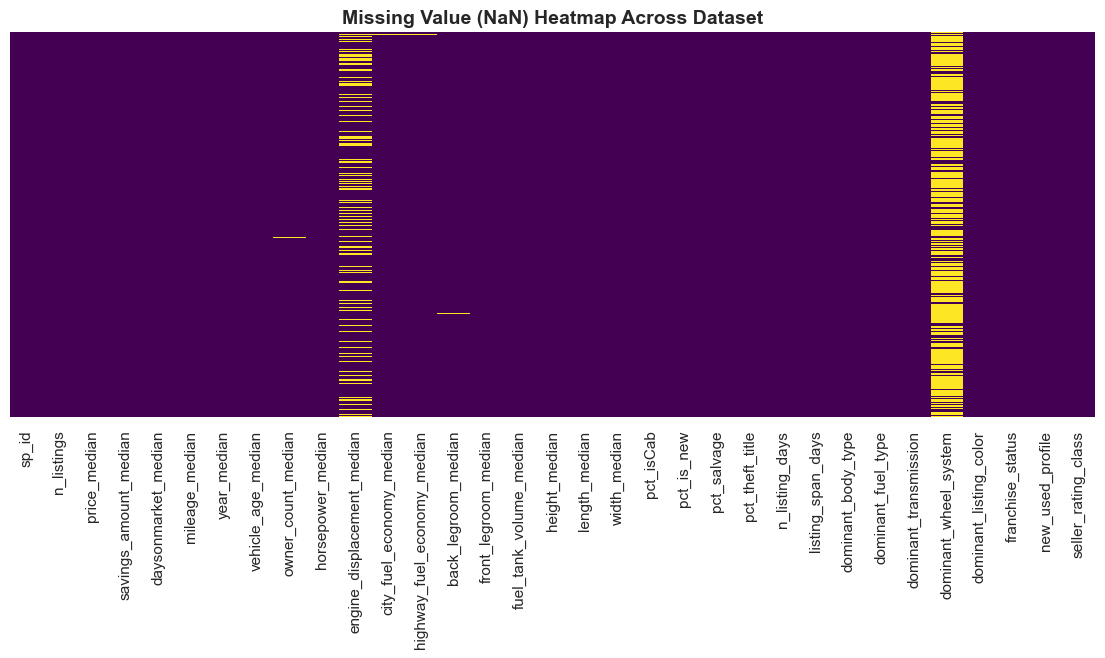
\includegraphics[width=\linewidth]{figures/fig_1_4_missing_heatmap.png}
  \caption{Missing-value (\texttt{NaN}) heatmap across the dataset.}
  \label{fig:missing}
\end{figure}

We applied tailored strategies to handle the missing values in each attribute:
\begin{itemize}[leftmargin=*]
  \item \texttt{dominant\_wheel\_system}: dropped due to the high percentage of missing values (75.98\%).
  \item \texttt{engine\_displacement\_median}: filled with the median grouped by \texttt{dominant\_body\_type} and \texttt{horsepower\_median} quintiles, ensuring that the engine size reflects both the vehicle's body type and power.
  \item \texttt{dominant\_listing\_color}: implicit \textit{unknown} values (10.91\%) are kept as a separate category, preventing mode substitution from over-representing the \textit{white} label.
  \item \texttt{dominant\_fuel\_type} and \texttt{dominant\_transmission}: the implicit \textit{unknown} values (1 and 6 instances) are replaced by the group mode computed across each \texttt{dominant\_body\_type}.
  \item \texttt{vehicle\_age\_median}: the single missing entry (0.01\%) was computed as $2020 - \texttt{year\_median}$.
  \item The remaining 14 numerical attributes (\texttt{owner\_count\_median}, \texttt{pct\_isCab}, \texttt{pct\_salvage}, \texttt{pct\_theft\_title}, physical dimensions, legrooms, fuel economy, \texttt{horsepower\_median} and \texttt{mileage\_median}): minor missing values ($<0.30\%$ each) are imputed using the group median across each \texttt{dominant\_body\_type}, preserving expected characteristics across body types.
\end{itemize}

\subsubsection{Outlier and noise detection}
\label{sec:outliers}
We used boxplots to spot the presence of possible outliers (Figure~\ref{fig:box}). Many attributes exhibit a significant amount of outliers, so we investigated each of them to distinguish true measurement noise from valid domain outliers.

\textbf{True semantic noise.} We identified 3 instances with \texttt{back\_legroom\_median} $= 0$ although their \texttt{dominant\_body\_type} is \texttt{suv\_crossover} or \texttt{sedan}. Since this is physically impossible, we converted these values to the group median by body type, as described in Section~\ref{sec:missing}.

\textbf{Valid domain outliers.} First, we examined \texttt{pct\_salvage} and \texttt{pct\_theft\_title}, which record 90.83\% and 84.56\% zeros, respectively. This results in $\mathrm{IQR}=0$, so any non-zero value is flagged as an outlier. However, these values represent valid second-hand or salvage dealerships rather than data errors, so we retained all records. Second, we examined extreme values across all attributes:
\begin{itemize}[leftmargin=*]
  \item \texttt{n\_listings} (up to 4,959) corresponds to a large-volume dealer.
  \item \texttt{price\_median} (up to \$236,438), \texttt{horsepower\_median} (up to 630 HP) and \texttt{vehicle\_age\_median} (up to 60 years) may correspond to luxury, sport or classic-car dealers.
  \item \texttt{city\_fuel\_economy\_median} (up to 126 MPG) represents electric-vehicle dealers.
  \item \texttt{daysonmarket\_median} (up to 1,987 days) reflects real market heterogeneity, as some dealers have slow-moving inventory.
\end{itemize}

We decided to keep all records from these valid sellers to retain niche market segments. The cleaned dataset therefore contains 13,843 records. We then applied logarithmic tail compression in Section~\ref{sec:transform}. For distance-sensitive models (such as K-Means), task-specific outlier filtering or robust scaling can be applied without altering the master dataset.

\begin{figure}[tbp]
  \centering
  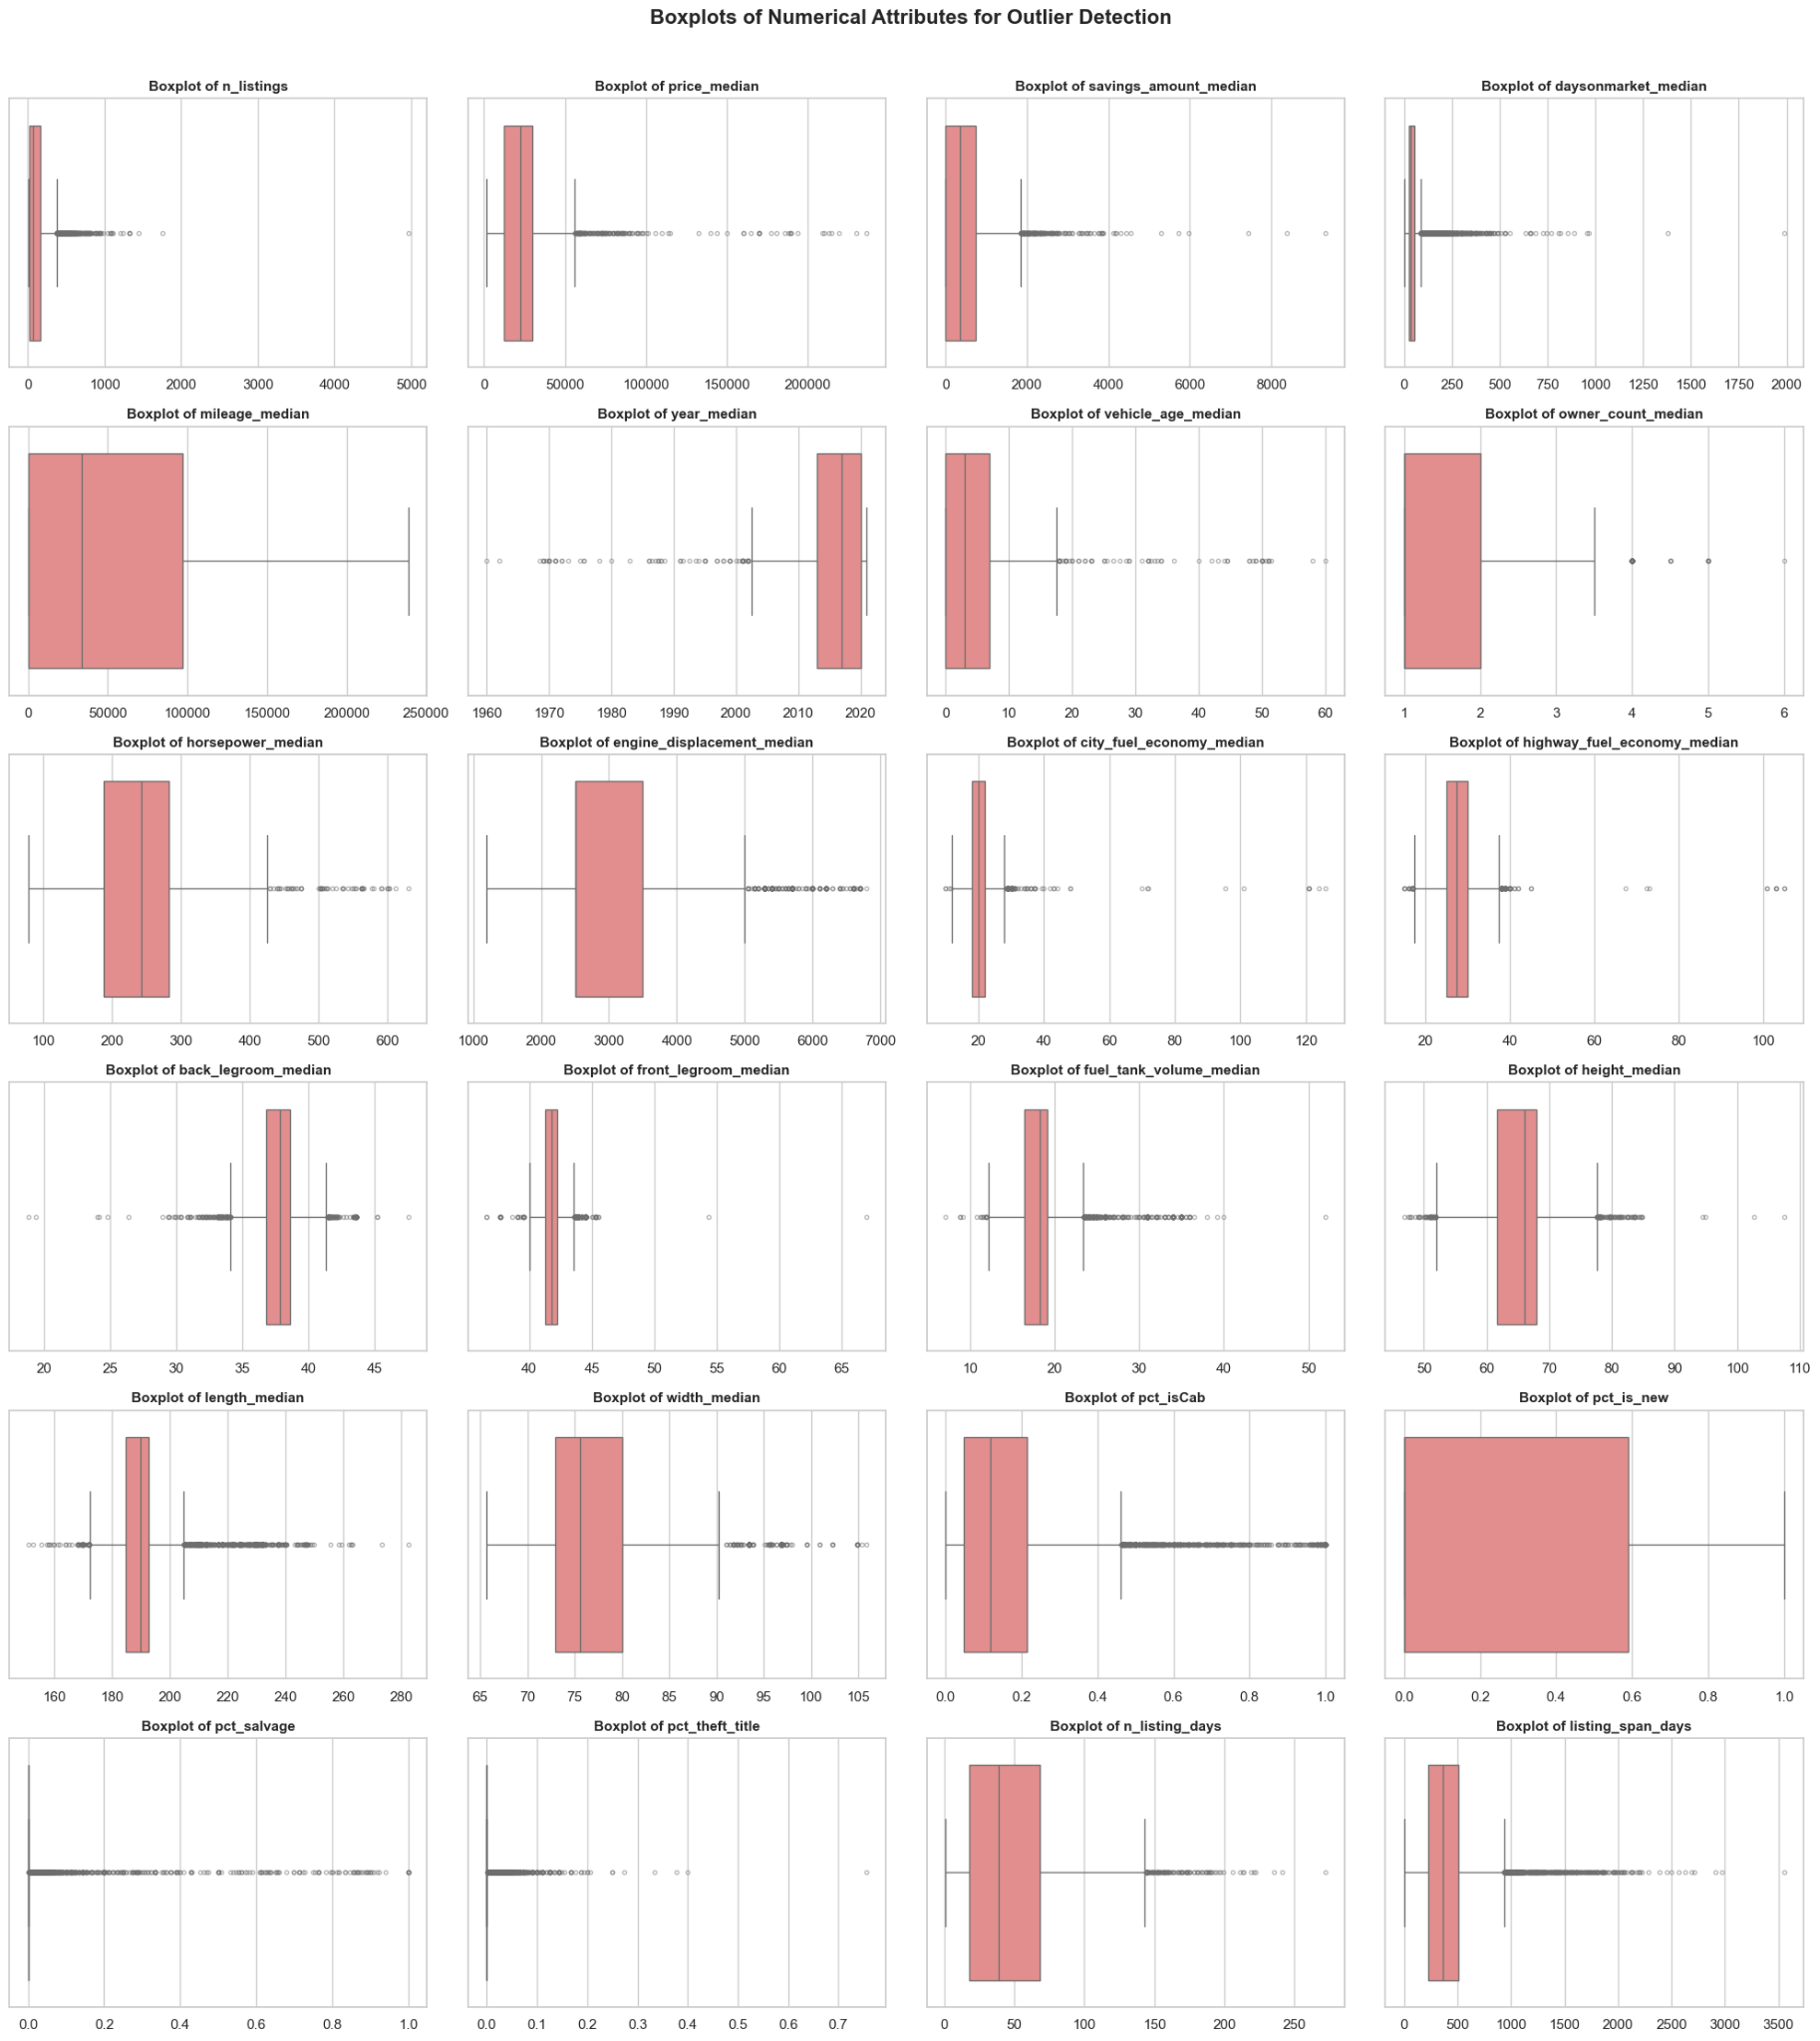
\includegraphics[width=0.75\linewidth]{figures/fig_1_5_boxplots.png}
  \caption{Boxplots of the numerical attributes for outlier detection.}
  \label{fig:box}
\end{figure}

\subsubsection{Variables transformation}
\label{sec:transform}
To address the heavy right skewness across the numerical attributes, we applied a logarithmic transformation, $\log(1+x)$, to the heavily right-skewed continuous features: \texttt{price\_median}, \texttt{n\_listings}, \texttt{daysonmarket\_median}, \texttt{savings\_amount\_median}, \texttt{vehicle\_age\_median}, \texttt{city\_fuel\_economy\_median}, \texttt{highway\_fuel\_economy\_median}, \texttt{engine\_displacement\_median} and \texttt{fuel\_tank\_volume\_median}. This compresses extreme right tails and restores near-symmetric distributions without undefined values at zero. We then performed feature scaling to ensure uniformity. We generated two standardised representations: Z-score standardisation to mitigate outlier leverage in distance-based algorithms, and Min-Max scaling for bounded metrics.

\subsubsection{Pairwise correlations and variable elimination}
\label{sec:correlations}
We analysed inter-feature dependencies across the numerical attributes using the pairwise scatter-plot matrix (Figure~\ref{fig:pairwise}) and the Spearman correlation matrix (Figure~\ref{fig:corr}). We selected Spearman over Pearson because Figure~\ref{fig:pairwise} reveals strong non-linear monotonic patterns; in particular, \texttt{price\_median} drops sharply as \texttt{mileage\_median} and \texttt{vehicle\_age\_median} increase and then flattens out, forming an L-shaped curve alongside the heavy right-tail outliers.

Careful observation of the correlation matrix reveals several important findings. First, regarding highly correlated pairs, we retained both \texttt{mileage\_median} and \texttt{vehicle\_age\_median} (0.93) as well as \texttt{n\_listings} and \texttt{n\_listing\_days} (0.96) in the master dataset, because their relative ratios capture annual vehicle usage and active posting intensity. Second, within the technical specifications, \texttt{engine\_displacement\_median} correlates positively with \texttt{fuel\_tank\_volume\_median} (0.79) and \texttt{horsepower\_median} (0.77), but negatively with \texttt{city\_fuel\_economy\_median} ($-0.76$), reflecting the trade-off between engine capacity and fuel efficiency.

Finally, we removed \texttt{year\_median} ($-0.98$ with \texttt{vehicle\_age\_median}, since the latter equals $2020 - \texttt{year\_median}$) and \texttt{highway\_fuel\_economy\_median} (0.94 with \texttt{city\_fuel\_economy\_median}, as they describe the same fuel efficiency). The final prepared dataset therefore contains 13,843 rows and 29 attributes.

\begin{figure}[H]
  \centering
  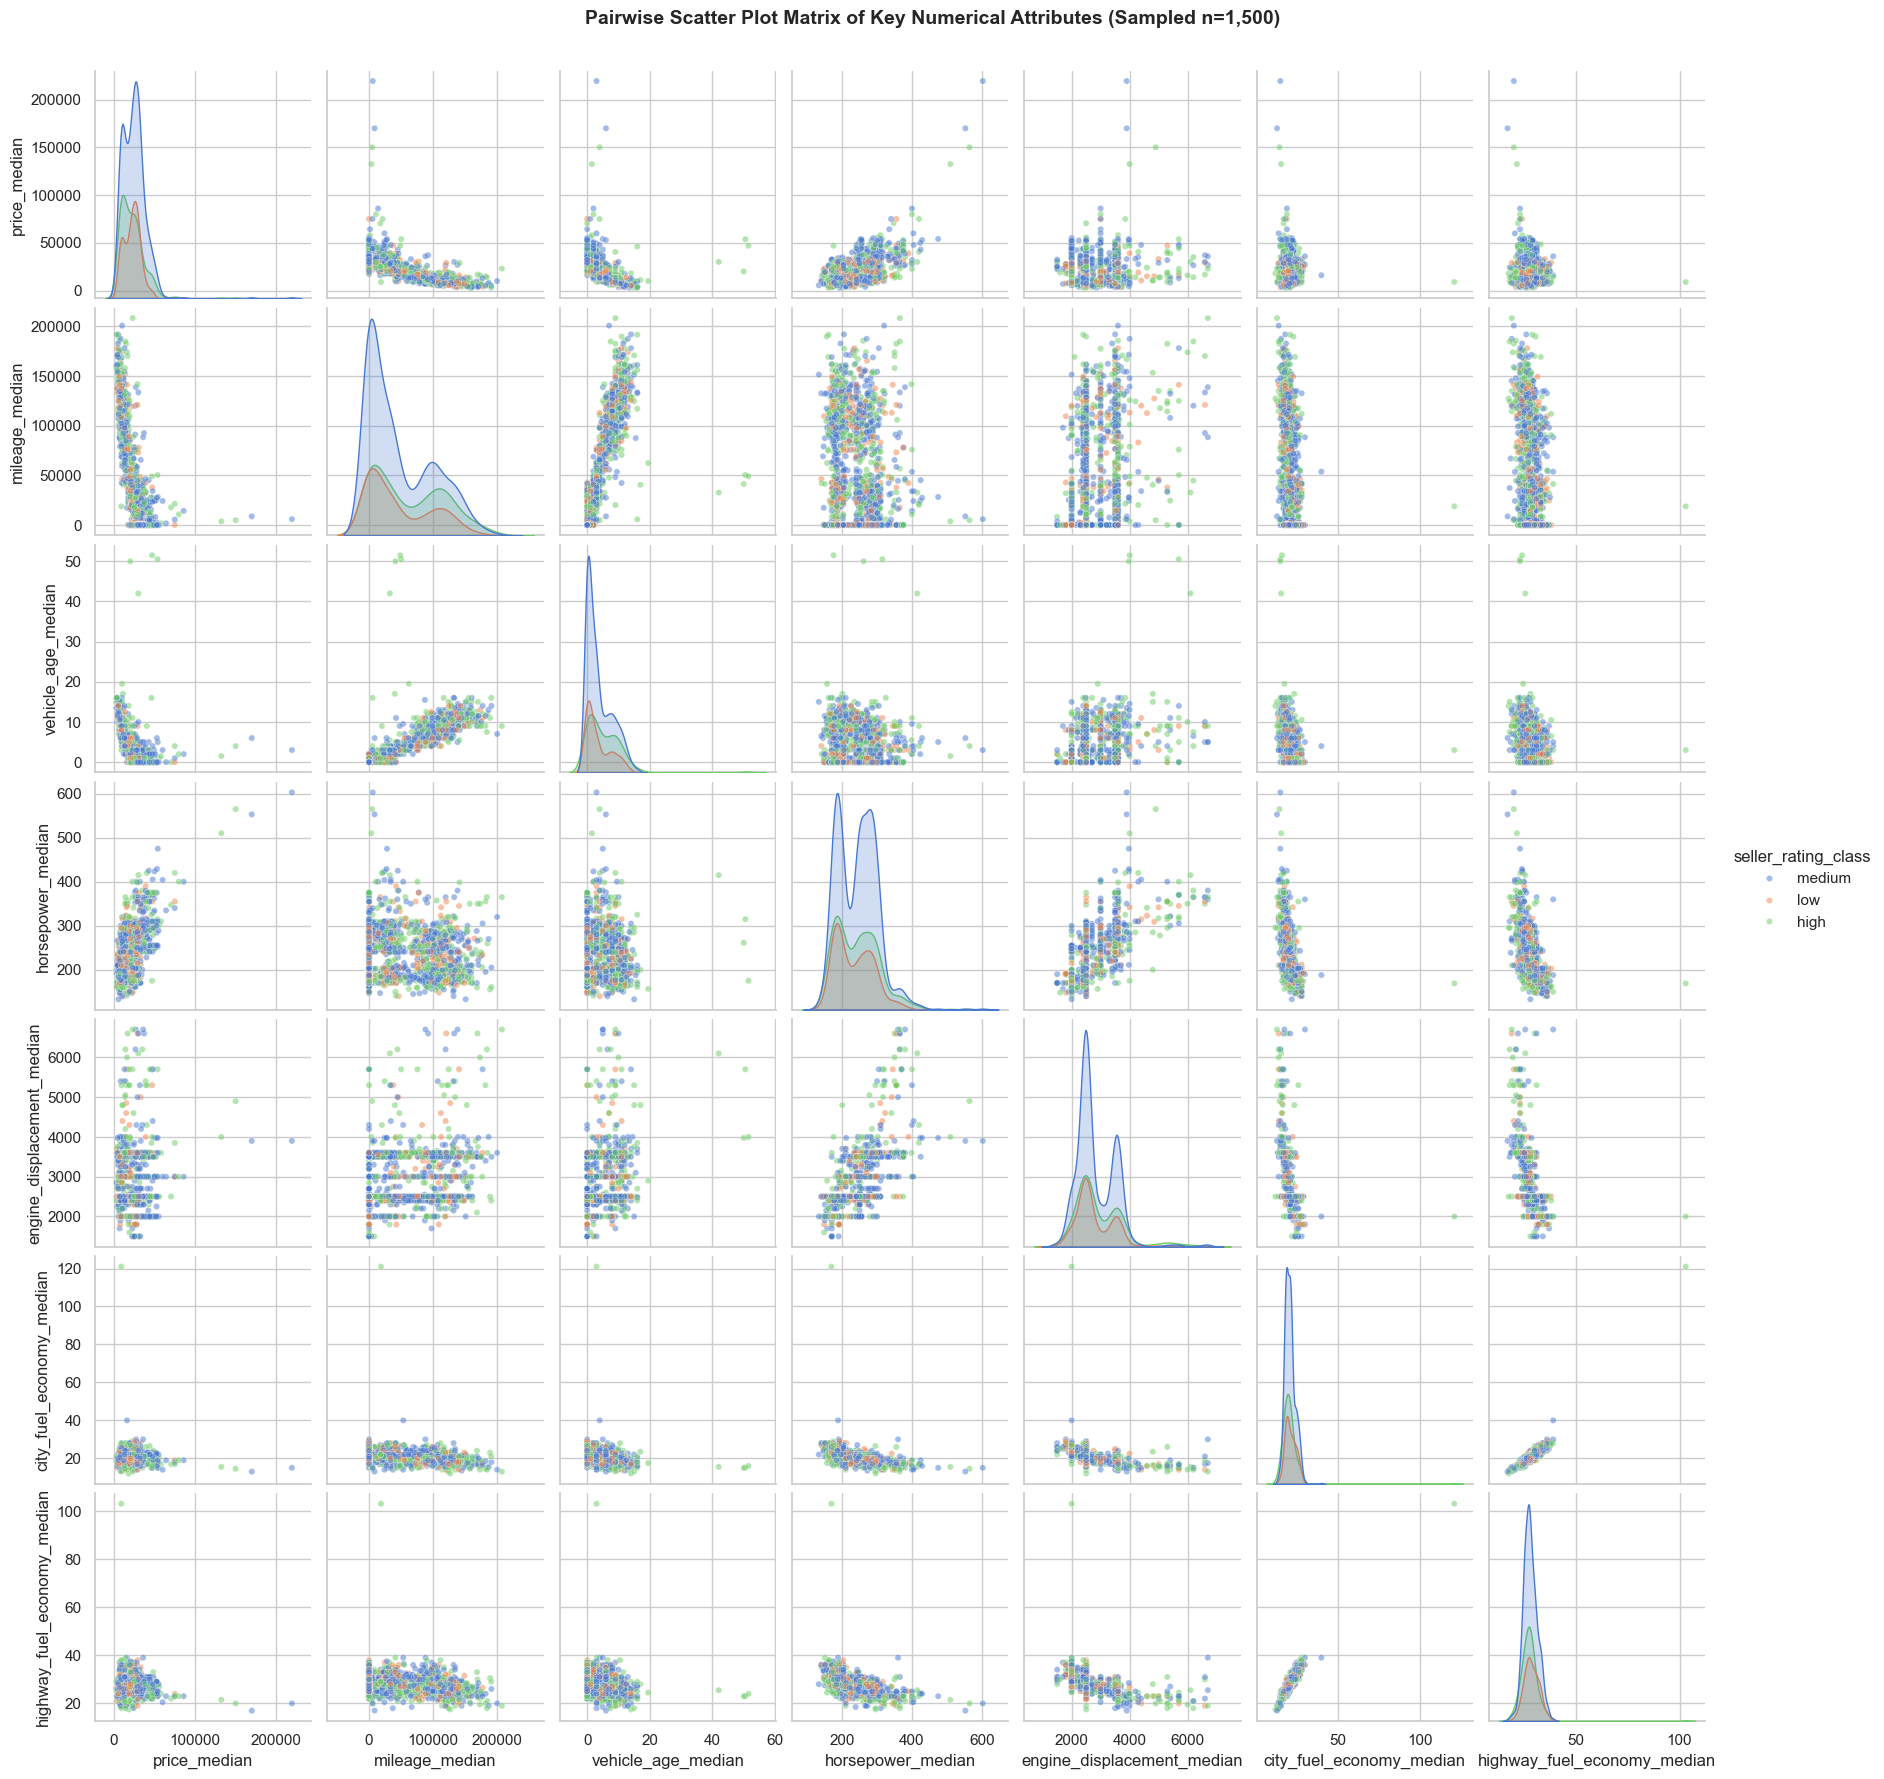
\includegraphics[width=0.62\linewidth]{figures/fig_1_6_pairwise.png}
  \caption{Pairwise scatter-plot matrix of the key numerical attributes (sampled).}
  \label{fig:pairwise}
\end{figure}

\begin{figure}[H]
  \centering
  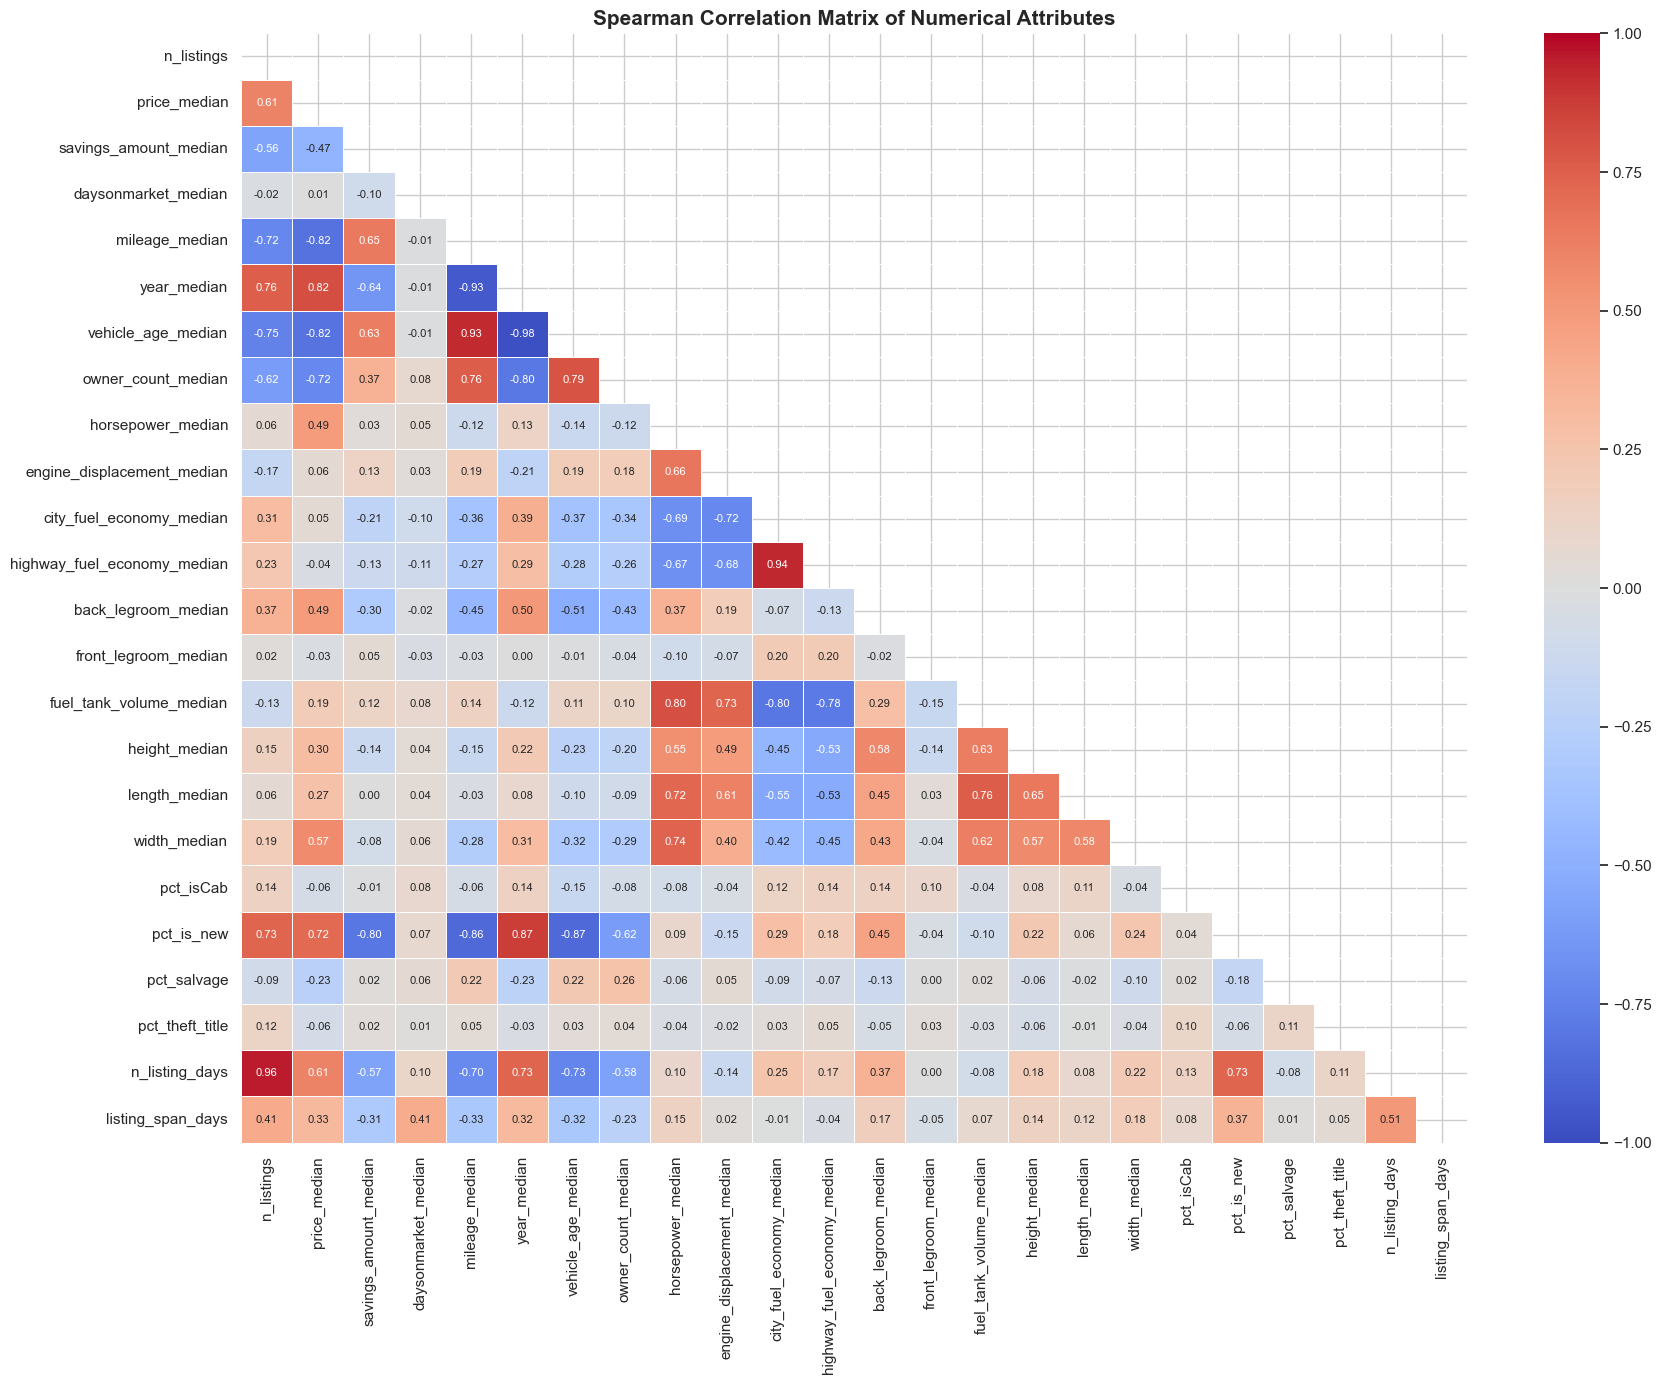
\includegraphics[width=0.62\linewidth]{figures/fig_1_7_correlation.png}
  \caption{Spearman correlation matrix of the numerical attributes.}
  \label{fig:corr}
\end{figure}

%=====================================================================
\section{Clustering}
\label{sec:clustering}
\emph{(TODO: describe the clustering setup, the features used, and how
dimensionality reduction was applied.)}

\subsection{Centroid-based}
\emph{(TODO: K-Means; elbow and silhouette for choosing $K$.)}

\subsection{Density-based}
\emph{(TODO: DBSCAN; $k$-NN distance plot to choose $\varepsilon$ and MinPts.)}

\subsection{Hierarchical}
\emph{(TODO: agglomerative clustering; linkage comparison and dendrograms.)}

\subsection{Final discussion}
\emph{(TODO: compare the methods and state which worked best.)}

%=====================================================================
\section{Classification}
\label{sec:classification}
The target variable is \texttt{seller\_rating\_class}. Describe the
preprocessing, the train/test split, and the evaluation metrics (accuracy,
precision, recall, F1, ROC-AUC).

\subsection{KNN}
\emph{(TODO: hyperparameter search results and per-class metrics.)}

\subsection{Na\"ive Bayes}
\emph{(TODO: Gaussian and/or Categorical Naive Bayes results.)}

\subsection{Decision Trees}
\emph{(TODO: tuning, pruning, and the resulting tree.)}

\subsection{Final conclusion}
\emph{(TODO: compare all classifiers and recommend one.)}

\begin{table}[h]
  \centering
  \caption{Model comparison. \emph{(Fill in.)}}
  \label{tab:clf-results}
  \small
  \begin{tabular}{lcccc}
    \toprule
    Model & Accuracy & Macro-F1 & Macro-AUC \\
    \midrule
    k-NN & & & \\
    Na\"ive Bayes & & & \\
    Decision Tree & & & \\
    \bottomrule
  \end{tabular}
\end{table}

%=====================================================================
\section{Regression}
\label{sec:regression}
\emph{(TODO: describe the regression target and predictors.)}

\subsection{Univariate regression}
\emph{(TODO: simple regression per predictor.)}

\subsection{Multivariate regression}
\emph{(TODO: multiple and multi-target regression.)}

%=====================================================================
\section{Pattern Mining}
\label{sec:patterns}
\emph{(TODO: describe the discretization/binning of numeric attributes and the
transactional representation.)}

\subsection{Frequent patterns}
\emph{(TODO: Apriori vs FP-Growth, support and itemset-size analysis.)}

\subsection{Association rules}
\emph{(TODO: top rules, support/confidence/lift, and interpretation.)}

%=====================================================================
\section{Conclusion}
\label{sec:conclusion}
\emph{(TODO: summarise the findings and the main takeaways.)}

\section*{Team Contributions}
\label{sec:contributions}
\begin{table}[h]
  \centering
  \small
  \begin{tabular}{p{0.3\linewidth}p{0.6\linewidth}}
    \toprule
    Member & Contribution \\
    \midrule
    \memberA & \\
    \memberB & \\
    \memberC & \\
    \bottomrule
  \end{tabular}
\end{table}

\end{document}
